\section{eo\-Uniform\-Init$<$ T $>$ Class Template Reference}
\label{classeo_uniform_init}\index{eoUniformInit@{eoUniformInit}}
The class eo\-Uniform\-Init can be used in the STL apply function to easily randomize floats and doubles.  


{\tt \#include $<$eo\-Uniform\-Init.h$>$}

Inheritance diagram for eo\-Uniform\-Init$<$ T $>$::\begin{figure}[H]
\begin{center}
\leavevmode
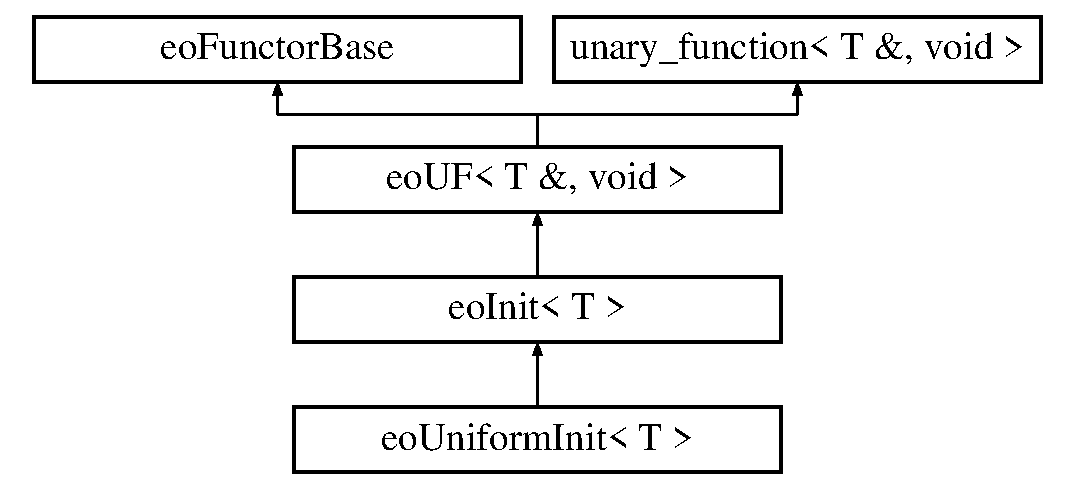
\includegraphics[height=4cm]{classeo_uniform_init}
\end{center}
\end{figure}
\subsection*{Public Member Functions}
\begin{CompactItemize}
\item 
{\bf eo\-Uniform\-Init} (T \_\-max=T(1.0), {\bf eo\-Rng} \&\_\-rng=rng)\label{classeo_uniform_init_a0}

\begin{CompactList}\small\item\em Ctor with only a max bound. \item\end{CompactList}\item 
{\bf eo\-Uniform\-Init} ({\bf eo\-Real\-Bounds} \&\_\-bound, {\bf eo\-Rng} \&\_\-rng=rng)\label{classeo_uniform_init_a1}

\begin{CompactList}\small\item\em Ctor with an eo\-Real\-Bound. \item\end{CompactList}\item 
{\bf eo\-Uniform\-Init} (T \_\-min, T \_\-max, {\bf eo\-Rng} \&\_\-rng=rng)\label{classeo_uniform_init_a2}

\begin{CompactList}\small\item\em Ctor with explicit min and max. \item\end{CompactList}\item 
void {\bf operator()} (T \&\_\-t)\label{classeo_uniform_init_a3}

\begin{CompactList}\small\item\em Generates the number, uses a static\_\-cast to get the right behaviour for ints and unsigneds. \item\end{CompactList}\item 
template$<$$>$ void {\bf operator()} (bool \&\_\-b)\label{classeo_uniform_init_a4}

\end{CompactItemize}
\subsection*{Private Attributes}
\begin{CompactItemize}
\item 
T {\bf minim}\label{classeo_uniform_init_r0}

\item 
T {\bf range}\label{classeo_uniform_init_r1}

\item 
{\bf eo\-Rng} \& {\bf uniform}\label{classeo_uniform_init_r2}

\end{CompactItemize}


\subsection{Detailed Description}
\subsubsection*{template$<$class T = double$>$ class eo\-Uniform\-Init$<$ T $>$}

The class eo\-Uniform\-Init can be used in the STL apply function to easily randomize floats and doubles. 

It can also be used for ints and unsigneds by virtue of the static\_\-cast

Also present is a specialization for boolean, that will ignore the minima and maxima that are possibly set and will return an unbiased flip of a coin. For a biased flip, use the eo\-Boolean

either in [0, \_\-max) if only 1 value (\_\-max) is given (or none, as \_\-max defaults to 1.0) or in [\_\-min,\_\-max) if 2 values are given (\_\-min, \_\-max) 



Definition at line 62 of file eo\-Uniform\-Init.h.

The documentation for this class was generated from the following file:\begin{CompactItemize}
\item 
eo\-Uniform\-Init.h\end{CompactItemize}
